\section{Diseño}

\subsection{planteamiento de circuito}
Para este laboratorio se plantea el siguiente diagrama de conexiones hecho en el software \texttt{Proteus}.
\begin{figure}[h!]
    \centering
    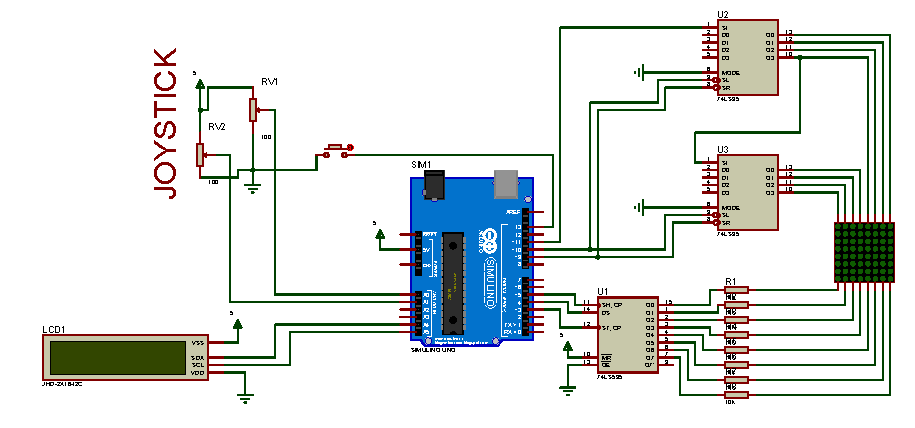
\includegraphics[width=0.9\textwidth]{Diagramas/xfcolor_cropped.pdf}
    \caption{Esquema de conexiones}
    \label{fig:esquema}
\end{figure}

Asi para el uso del registro de desplazamiento 74HC595 de 8 bits, se conectan 3 pines digitales hacia el integrado, siendo uno para enviar los datos en serie 
hacia el registro, otro para el reloj y el ultimo para el control del latch. La salida de este integrado se conecta a 8 resistencias de $\SI{220}{\ohm}$
para limitar la corriente de estos pines, finalmente este se conecta a la matriz LED 8x8. Tambien se utiliza el pin de alimentacion de $\i$

Para los registros de desplazamiento de 4 bits, estos se tiene que conectar en cascada, para poder formar los 8 bits necesarios para controlar la matriz led.
Asi se utilizan 3 pines digitales para esta conexion

\subsection{Desarrollo del código}
El código se estructuró para gestionar simultáneamente las entradas del joystick, la lógica del juego (movimiento y colisiones), y el refresco de las salidas (matriz LED y LCD). El principio fundamental de diseño fue descargar el proceso de multiplexado de la matriz del ciclo principal (\texttt{loop()}) a las interrupciones por tiempo, permitiendo que el \texttt{loop()} se dedicara exclusivamente a la lógica del juego.




\subsubsection*{1. Optimización de Memoria con Campos de Bits}

Para gestionar la posición del cazador (\texttt{player}) y el blanco (\texttt{goal}), se utilizó una estructura de datos \texttt{pos} que emplea \textbf{campos de bits} (bit fields):

Dado que la matriz es de $8\times8$ LEDs, las coordenadas X e Y solo necesitan valores de 0 a 7, lo que se puede representar con 3 bits ($2^3=8$). Esta técnica permitió empaquetar ambas coordenadas en un solo byte (6 bits utilizados), logrando una gestión de memoria muy eficiente.

El fragmento de código relevante es:

    \begin{minted}{cpp}
// Posición del cazador y del blanco (usando 3 bits por coordenada para ahorrar memoria)
struct pos {
  byte x : 3;
  byte y : 3;
} player, goal;
    \end{minted}


\subsubsection*{2. Estructura de la Matriz y Manipulación Bitwise}

El estado visual del juego se mantiene en el arreglo de 8 bytes \texttt{matrix[8]}, donde cada byte representa el estado de una columna de la matriz LED. Esta representación es clave para la eficiencia de las actualizaciones.

\begin{itemize}
    \item \textbf{Estructura Lógica:} \texttt{matrix[Y]} almacena los 8 LEDs de la columna $Y$. Un bit encendido (\texttt{1}) significa que el LED en esa posición debe estar activo.
    \item \textbf{Operaciones de Bits:} Las actualizaciones de posición (\texttt{player}) y el parpadeo (\texttt{goal}) se realizan mediante operaciones a nivel de bit. El índice de la matriz se ajusta dinámicamente utilizando el operador ternario (\texttt{?:}) para compensar la configuración física del cableado de la matriz.
    \begin{itemize}
        \item \textbf{Encender/Actualizar:} Se utiliza la operación OR  para establecer el bit de la nueva posición del cazador en 1.
        \item \textbf{Borrar/Parpadear :} Se utiliza la operación XOR para invertir el estado del bit. Esto se usa tanto para el parpadeo del blanco como para borrar la posición anterior del cazador.
    \end{itemize}
\end{itemize}



    \begin{minted}{cpp}
// Cada 250ms leer entrada y mover al cazador
// También se hace parpadear al blanco
if (millis() - poll_time >= 250) {
  poll_time = millis();

  val_x = analogRead(JOY_X);
  val_y = analogRead(JOY_Y);

  // Borrar punto de cazador anterior.
  matrix[player.y == 0 ? 7 : (player.y - 1)] ^= (1 << player.x);

   // Zona muerta de 256, o 50% de la resolución
      // Sólo se actualiza la posición si no se va a chocar con la pared o el borde
      if (val_x < 256 && (player.x > 0 && !(player.x == 5 && (player.y == 3 || player.y == 4)))) player.x -= 1;
      else if (val_x > 768 && (player.x < 7 && !(player.x == 2 && (player.y == 3 || player.y == 4)))) player.x += 1;
      if (val_y < 256 && (player.y < 7 && !(player.y == 2 && (player.x == 3 || player.x == 4)))) player.y += 1;
      else if (val_y > 758 && (player.y > 0 && !(player.y == 5 && (player.x == 3 || player.x == 4)))) player.y -= 1;


  // Actualizar bits en la matriz con la nueva posición
  matrix[player.y == 0 ? 7 : (player.y - 1)] |= (1 << player.x);

  // Parpadeo del blanco (cambiar su estado con XOR)
  matrix[goal.y == 0 ? 7 : (goal.y - 1)] ^= (1 << goal.x);
}
\end{minted}


     

\subsubsection*{3. Control de Refresco mediante Interrupciones (Timer1)}

El refresco de la matriz LED, es importante para evitar el efecto de parpadeo, se implementó usando el Timer1 del microcontrolador. Esto garantiza que la actualización sea periódica y no dependa del tiempo de ejecución del \texttt{loop()}. Se configuraron dos interrupciones (ISRs):

\begin{itemize}
    \item \textbf{\texttt{ISR(TIMER1\_COMPA\_vect)}}: Se ejecuta a 2500 Hz. Es la responsable de \textbf{desactivar} la fila actual para prevenir ela persistencia de la imagen anterior, e inmediatamente carga los datos de columna (\texttt{DCOL}) para la \textit{siguiente} fila a dibujar.

    \item \textbf{\texttt{ISR(TIMER1\_COMPB\_vect)}}: Se ejecuta a 5000 Hz, actuando 200 $\mu$s después de la interrupción A. Su función es \textbf{activar} la fila correspondiente al \texttt{counter} actual, encendiendo así la fila con los datos de columna previamente cargados.
\end{itemize}


La configuración del temporizador en \texttt{setup()} y los ISRs son:


    \begin{minted}{cpp}
// -- Configuración de interrupts de tiempo (Timer1 para multiplexado de matriz) --
  TCCR1A = 0; // Limpiar registros A
  TCCR1B = 0; // Limpiar registros B
  // ... (otros registros de configuración de Timer1)
  TIMSK1 |= (1 << OCIE1A) | (1 << OCIE1B);
  OCR1A = 6400; // Valor de comparación A (400us)
  OCR1B = 3200; // Valor de comparación B (200us)
// -------------------------------------------
ISR(TIMER1_COMPA_vect) {
  // 1. Deshabilitar la fila actual (blanquear) para evitar ghosting
  digitalWrite(LROW, LOW);
  shiftOut(DROW, CLK1, LSBFIRST, 0x00);
  // ...
}
ISR(TIMER1_COMPB_vect) {
  // 1. Activar la fila 'counter' 
  digitalWrite(LROW, LOW);
  shiftOut(DROW, CLK1, LSBFIRST, (1 << counter));
  digitalWrite(LROW, HIGH);
}
    \end{minted}


\subsubsection*{4. Lógica del Juego y Detección de Colisión}

La función \texttt{loop()} se encarga de la lógica principal:

\vspace{1em}
\begin{enumerate}
    \item \textbf{Polling del Joystick:} La lectura de las entradas analógicas (\texttt{JOY\_X}, \texttt{JOY\_Y}) se realiza cada $250\text{ms}$ para un movimiento controlado, estableciendo una zona muerta para evitar movimientos involuntarios.
    \item \textbf{Actualización y Colisión:} Se calcula la nueva posición del jugador, aplicando reglas de detección de colisión que impiden que el cazador se mueva sobre las coordenadas fijas del muro ($x=3, 4$ y $y=3, 4$). La posición se actualiza en el arreglo \texttt{matrix} utilizando operaciones de bits (\texttt{OR} para encender, \texttt{XOR} para borrar la posición anterior).
    \item \textbf{Fin de Partida:} Se evalúan dos condiciones de término: victoria (cuando \texttt{player} y \texttt{goal} coinciden) y derrota por tiempo límite ($5\text{s}$), actualizando el estado del juego (\texttt{game\_state}) y la pantalla LCD.
\end{enumerate}

El control de movimiento en \texttt{loop()} incluye una lógica de colisión para evitar que el cazador se mueva a las posiciones ocupadas por el muro estático. Por ejemplo, la prevención de movimiento a la derecha (\texttt{player.x += 1}) cuando se está justo a la izquierda del muro:

    \begin{minted}{cpp}
        // Choque a la DERECHA: player.x = 2, y el movimiento es a la derecha (hacia columna 3 o 4)
else if (val_x > 768 && player.x < 7) { 
  if (!((player.x == 2) && (player.y == 3 || player.y == 4))) player.x += 1;
}
    \end{minted}


